\section{Définition}
L'OCR ou encore la reconnaissance optique de caractères est une technologie complexe qui convertit les images contenant du texte en formats avec du texte modifiable. Il permet de traiter des livres numérisés, des captures d'écran et des photos contenant du texte et d'obtenir des documents modifiables tels que des fichiers TXT, DOC ou PDF.
\begin{figure}[H]
    \centering
    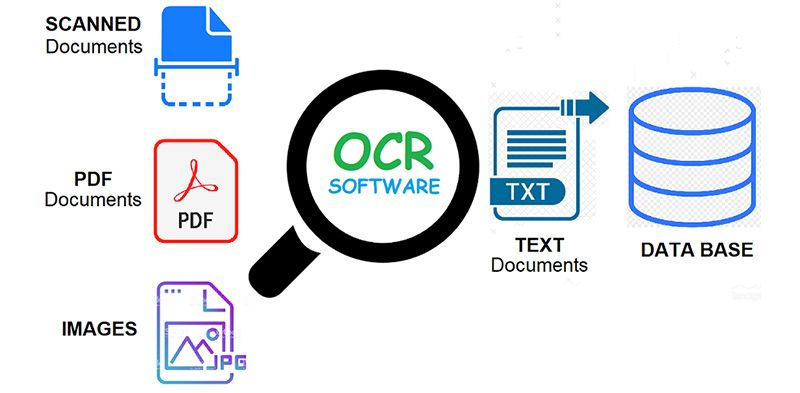
\includegraphics[scale=0.25]{OCR}
    \caption{Processus d'OCR}
\end{figure}